


\begin{document}
	
This report describes the design, construction, and analysis of negative feedback for an operational amplifier. This is achieved using  resistors attached to and across certain nodes in the op amp in Figure \ref{fig:sample}


\begin{figure}[H]
	\begin{center}
		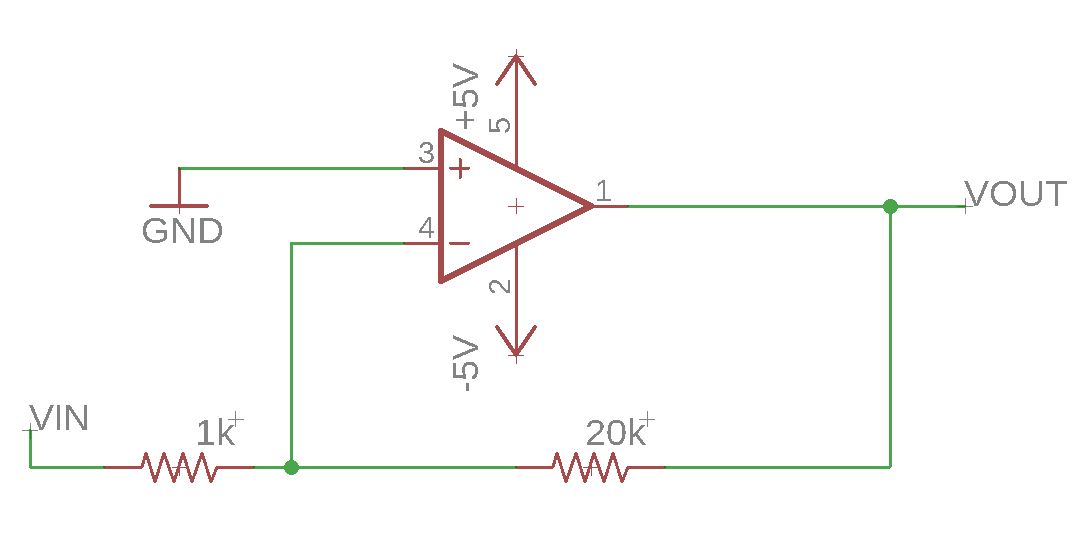
\includegraphics[scale=.40]{Introduction/invertingschem.png}
		\caption{Sample experimental circuit demonstrating feedback}
		\label{fig:sample}
	\end{center}
\end{figure}
	
	
	
	
	
Operational amplifiers serve an integral building block for modern electronics. Op amps provide large gain with various configuration schema. This allows the circuit designer to use the op amp in different topologies and achieve different results, all without modifying the op amp circuit itself. In addition, an op amp provides significant gain while maintaining stability, this is where the output stage comes in. The output stage allows design to accommodate for non-controllable factors such as transistor mismatch and temperature variation.   The objective of this lab is to apply feedback to the op amp so that the op amp achieves the specifications as seen in Table \ref{tab:labspecs}

\begin{table}[H]
	\centering
	\caption{Task 5 Specifications}
	\label{tab:labspecs}
	\begin{tabular}{|c|c|}
			\hline
			\textbf{Specifications} &                 \\ \hline
			Power                   & $\pm$5V         \\ \hline
			Output Stage 			& $\geq$ 500$\Omega$ \\ \hline
			Bias Current            & 400 $\mu$A      \\ \hline
			Overall Voltage Gain    & $\geq$200V/V (46 dB)  \\ \hline
			CMRR                    & $\geq$ 60dB     \\ \hline
			Output Voltage Swing    & $\geq$ $\pm$ 2V \\ \hline
		\end{tabular}
\end{table}

\noindent Section 2 of this report describes the design, and when relevant, the simulations of the experiments. Experimental results and implementation are addressed in Section 3, including reasoning as to why a different circuit than the one outlined previously was constructed. A discussion of the results, sources of error, and areas of possible improvement are outlined in Section 4. Section 5 concludes this report. \newline


\end{document}